% Options for packages loaded elsewhere
\PassOptionsToPackage{unicode}{hyperref}
\PassOptionsToPackage{hyphens}{url}
%
\documentclass[
  12pt,
]{article}
\title{\vspace{5cm}

Predicting Vaccine Hesitancy for Humana Members}
\author{2021 Humana-Mays Healthcare Analytics Case Competition}
\date{October 10, 2021}

\usepackage{amsmath,amssymb}
\usepackage{lmodern}
\usepackage{iftex}
\ifPDFTeX
  \usepackage[T1]{fontenc}
  \usepackage[utf8]{inputenc}
  \usepackage{textcomp} % provide euro and other symbols
\else % if luatex or xetex
  \usepackage{unicode-math}
  \defaultfontfeatures{Scale=MatchLowercase}
  \defaultfontfeatures[\rmfamily]{Ligatures=TeX,Scale=1}
\fi
% Use upquote if available, for straight quotes in verbatim environments
\IfFileExists{upquote.sty}{\usepackage{upquote}}{}
\IfFileExists{microtype.sty}{% use microtype if available
  \usepackage[]{microtype}
  \UseMicrotypeSet[protrusion]{basicmath} % disable protrusion for tt fonts
}{}
\usepackage{xcolor}
\IfFileExists{xurl.sty}{\usepackage{xurl}}{} % add URL line breaks if available
\IfFileExists{bookmark.sty}{\usepackage{bookmark}}{\usepackage{hyperref}}
\hypersetup{
  pdfauthor={2021 Humana-Mays Healthcare Analytics Case Competition},
  hidelinks,
  pdfcreator={LaTeX via pandoc}}
\urlstyle{same} % disable monospaced font for URLs
\usepackage[margin=1.25in]{geometry}
\usepackage{graphicx}
\makeatletter
\def\maxwidth{\ifdim\Gin@nat@width>\linewidth\linewidth\else\Gin@nat@width\fi}
\def\maxheight{\ifdim\Gin@nat@height>\textheight\textheight\else\Gin@nat@height\fi}
\makeatother
% Scale images if necessary, so that they will not overflow the page
% margins by default, and it is still possible to overwrite the defaults
% using explicit options in \includegraphics[width, height, ...]{}
\setkeys{Gin}{width=\maxwidth,height=\maxheight,keepaspectratio}
% Set default figure placement to htbp
\makeatletter
\def\fps@figure{htbp}
\makeatother
\setlength{\emergencystretch}{3em} % prevent overfull lines
\providecommand{\tightlist}{%
  \setlength{\itemsep}{0pt}\setlength{\parskip}{0pt}}
\setcounter{secnumdepth}{5}
\newlength{\cslhangindent}
\setlength{\cslhangindent}{1.5em}
\newlength{\csllabelwidth}
\setlength{\csllabelwidth}{3em}
\newlength{\cslentryspacingunit} % times entry-spacing
\setlength{\cslentryspacingunit}{\parskip}
\newenvironment{CSLReferences}[2] % #1 hanging-ident, #2 entry spacing
 {% don't indent paragraphs
  \setlength{\parindent}{0pt}
  % turn on hanging indent if param 1 is 1
  \ifodd #1
  \let\oldpar\par
  \def\par{\hangindent=\cslhangindent\oldpar}
  \fi
  % set entry spacing
  \setlength{\parskip}{#2\cslentryspacingunit}
 }%
 {}
\usepackage{calc}
\newcommand{\CSLBlock}[1]{#1\hfill\break}
\newcommand{\CSLLeftMargin}[1]{\parbox[t]{\csllabelwidth}{#1}}
\newcommand{\CSLRightInline}[1]{\parbox[t]{\linewidth - \csllabelwidth}{#1}\break}
\newcommand{\CSLIndent}[1]{\hspace{\cslhangindent}#1}
\usepackage{setspace} \doublespacing \setlength{\parskip}{2mm} \usepackage{float} \floatplacement{figure}{H} \usepackage[skip=4pt]{caption}
\usepackage{booktabs}
\usepackage{longtable}
\usepackage{array}
\usepackage{multirow}
\usepackage{wrapfig}
\usepackage{float}
\usepackage{colortbl}
\usepackage{pdflscape}
\usepackage{tabu}
\usepackage{threeparttable}
\usepackage{threeparttablex}
\usepackage[normalem]{ulem}
\usepackage{makecell}
\usepackage{xcolor}
\ifLuaTeX
  \usepackage{selnolig}  % disable illegal ligatures
\fi

\begin{document}
\maketitle

\newpage
\tableofcontents

\newpage

\hypertarget{executive-summary}{%
\section{Executive Summary}\label{executive-summary}}

This study was a statistical data investigation into COVID-19
vaccination status for Humana members. In particular, our main goal was
to build a predictive model for identifying which members are most
likely to be hesitant to the COVID-19 vaccine. Furthermore, we wanted to
provide recommendations and potential solutions to increase vaccination
rates among the sub-segments of hesitant members based on the insights
obtained from the data.

In this work, we implemented two boosted tree classification methods,
namely, XGBoost and CatBoost, to predict vaccination status for Humana
members and identify important variables that contribute the most to the
predictions. After preprocessing the data and training the models, we
found that CatBoost was the best classifier in terms of maximizing the
area under a receiver operating characteristic (ROC) curve (AUC). In
addition, we obtained from our best model that Member Age and Race were
the two most significant predictors for explaining the likelihood of
vaccine hesitancy.

Then, based on our observations, we recommended that Humana distributes
pamphlets and surveys, utilizes peer-to-peer communication, and performs
joint-intervention with pharmacies to target those refusing the vaccine.
By implementing our recommendations based on the model predictions, key
indicators, and relevant research, Humana will be able to achieve its
goal of increasing the COVID-19 vaccination rate among their members.

\newpage

\hypertarget{background}{%
\section{Background}\label{background}}

Humana is a leading healthcare company that offers a wide range of
insurance products and health and wellness services. Their mission is
simply to help people achieve lifelong well-being. In addition, with the
current COVID-19 pandemic, increasing the vaccination rates among the
members of Humana remains to be the top priority for both members as
well as the larger population. They are primarily focused on providing
vaccination opportunities for the most vulnerable and underserved
populations. Thus, the objective of this study is to help Humana
identify which members are likely to be hesitant so that they could
design targeted outreaches for these individuals.

Extending into nearly every field from sports, education, to general
healthcare, vaccine hesitancy is an issue that has crept into the minds
of people beyond the business sector. Nearly 80\% of the unvaccinated
are unlikely to change their minds about getting a vaccine (Jones,
2021), highlighting the importance of addressing vaccine confidence
today. Our goal is to build a predictive model using observed
characteristics provided by the data to estimate the probability of
being hesitant to receive the COVID-19 vaccine for each member. More
importantly, with the use of these probabilities, features, and
statistical analysis, we wanted to provide recommendations and potential
solutions to drive vaccination among the sub-segments of hesitant
members.

\newpage

\hypertarget{data}{%
\section{Data}\label{data}}

The training dataset provided for this study contains a total of 974,842
rows and 368 columns in which information on medical claims, pharmacy
claims, lab claims, demographic/consumer data, credit data,
condition-related features, CMS features, and other features were
included. Our target variable, \texttt{covid\_vaccination} indicates the
vaccination status of each member. Vaccinated members were coded as
\texttt{vacc} and unvaccinated members were coded as \texttt{no\_vacc}.

We first wanted to reduce the size of our data, in particular, the
number of columns. For instance, we filtered out variables with
(near)-zero variance to eliminate potential problems with model
stability. In addition, we repaired categorical variables that were
misrepresented as numeric features when the data was imported. This left
us with 311 total independent variables and 1 column for the response
variable - whether or not a member is vaccinated.

After cleaning up the data, we summarized the COVID vaccination status
for members and looked for trends among various predictors. First, we
looked at the relationship between whether or not a member is vaccinated
versus age and gender. We decided to convert age, which was originally a
continuous variable, into discrete intervals (bins), for the purpose of
exploratory analysis only. The age groups that we partitioned age into
are 20-55, 55-65, 65-75, and 75+. We could see from Figure 1 that older
members tend to have higher vaccination rate than younger members.
Moreover, within each age group, the vaccination percentage is higher
for female members than the male group.

\begin{figure}[H]

{\centering 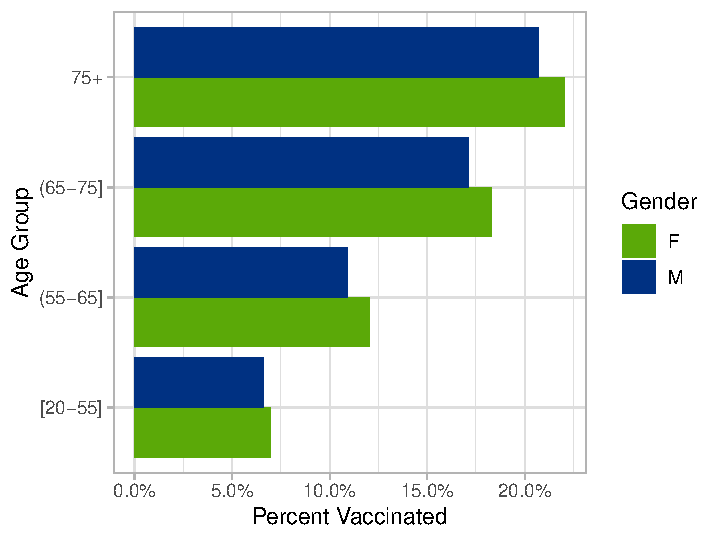
\includegraphics{report_files/figure-latex/unnamed-chunk-3-1} 

}

\caption{Bar graph of percent vaccinated by age group, color coded by gender.}\label{fig:unnamed-chunk-3}
\end{figure}

Another variable we wanted to explore is race. More than 80\% of the
members in the original data were identified as White, with the rest
being Black, Other, Asian, Hispanic, North American Native, or Unknown.
Figure 2 tells us that members with race codes 5, 6, and 2, which are
Hispanic, North American Native, and Black, respectively, have lower
vaccination rate than other race groups.

In addition, we looked at the association between vaccination status and
the original reason for entry into medicare (ResDAC, 2021). According to
Figure 3, members who entered Medicare because of Old Age Survivors
Insurance (OASI, coded 0) obtained the highest vaccination rate out of
all the other reasons (Disability Insurance Benefits (DIB), End-stage
Renal Disease (ESRD), or both - coded 1, 2, and 3).

\begin{figure}[H]

{\centering 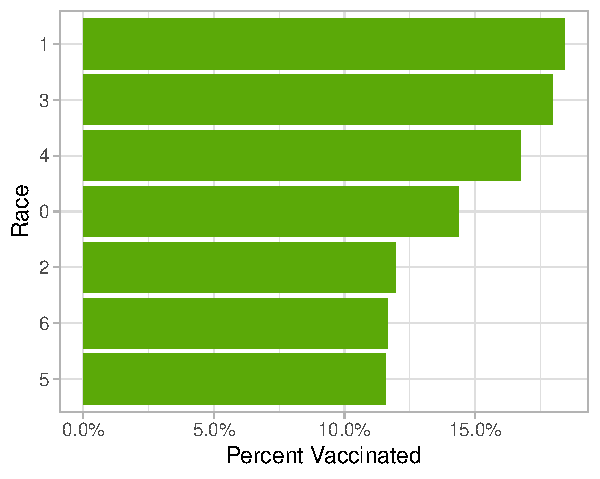
\includegraphics{report_files/figure-latex/unnamed-chunk-4-1} 

}

\caption{Bar graph of percent vaccinated by race. The race code values are: 0 = Unknown; 1 = White; 2 = Black; 3 = Other; 4 = Asian; 5 = Hispanic; 6 = North American Native}\label{fig:unnamed-chunk-4}
\end{figure}

\begin{figure}[H]

{\centering 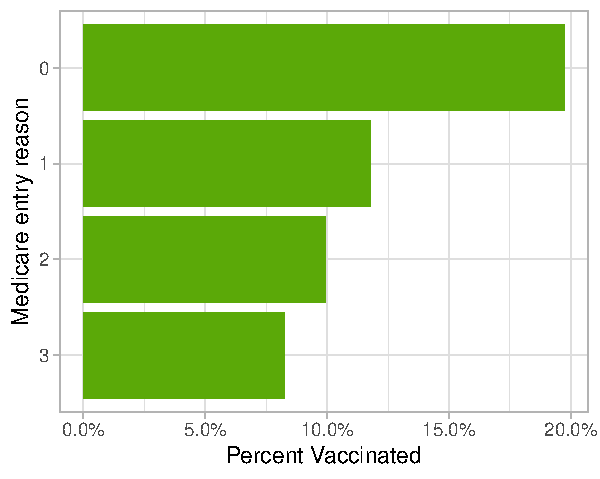
\includegraphics{report_files/figure-latex/unnamed-chunk-5-1} 

}

\caption{Bar graph of percent vaccinated by original reason for entry into Medicare. The original reason for Medicare entitlement code values are: 0    = Old age and survivor’s insurance (OASI); 1 = Disability insurance benefits (DIB); 2 = End-stage renal disease (ESRD); 3   = Both DIB and ESRD}\label{fig:unnamed-chunk-5}
\end{figure}

\newpage

\hypertarget{predictive-models}{%
\section{Predictive Models}\label{predictive-models}}

In this section, we presented our models for predicting vaccine
hesitancy for Humana members. To tackle this prediction problem, we
considered the following supervised machine learning techniques: XGBoost
(eXtreme Gradient Boosting) and CatBoost. To evaluate the performance of
the classfiers, the metric that we used was area under the receiver
operating characteristic curve (ROC/AUC).

\hypertarget{xgboost}{%
\subsection{XGBoost}\label{xgboost}}

The first model we considered was gradient boosted trees using the
popular eXtreme Gradient Boosting (XGBoost) method (Chen \& Guestrin,
2016). We implemented XGBoost via the \texttt{xgboost} package (Chen et
al., 2021) and with the \texttt{tidymodels} framework (Kuhn \& Wickham,
2020) in the \texttt{R} programming language (R Core Team, 2021). To get
the data into a useful format, median imputation was performed on
numeric variables with missing data, while an ``unknown'' level
representing missing values was added to the categorical covariates. We
also implemented one-hot encoding to turn our qualitative predictors
into indicator columns.

After that, we trained our XGBoost model on a 75-25 train-test split,
with 3-fold cross-validation. Our final XGBoost model consisted of the
following hyperparameters: learning rate of 0.02, 1150 trees, and a
number of predictors sampled for spliting at each node of 6. We then
made predictions on the validation set and obtained an ROC/AUC score of
0.6727 from this XGBoost fit (see Figure 4).

\begin{figure}[H]

{\centering 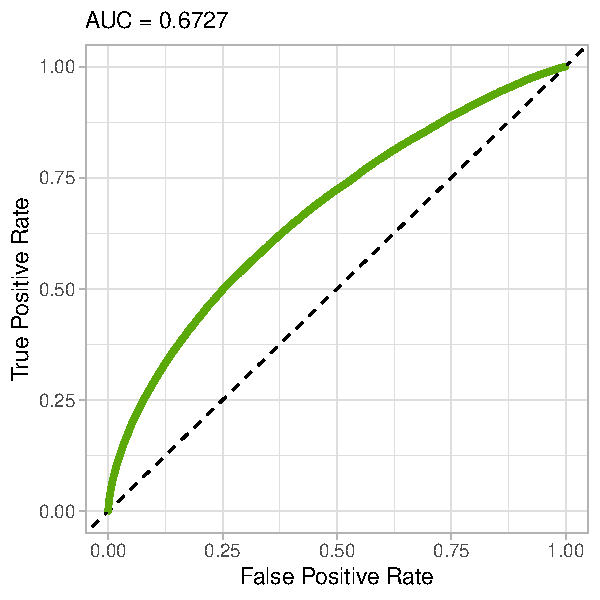
\includegraphics{report_files/figure-latex/unnamed-chunk-6-1} 

}

\caption{Receiver operating characteristic curve for XGBoost classification performance on the validation set.}\label{fig:unnamed-chunk-6}
\end{figure}

\hypertarget{catboost}{%
\subsection{CatBoost}\label{catboost}}

In addition, we explored another gradient boosting framework, CatBoost
(Prokhorenkova et al., 2018), provided by the \texttt{catboost}
\texttt{R} package. The advantage of using CatBoost is that minimal data
preparation is required. This algorithm handles missing values for
numeric features and non-encoded categorical features. The only data
mutating steps we performed were turning the response
(\texttt{covid\_vaccination}) into a binary indicator with 0 =
\texttt{vacc} and 1 = \texttt{no\_vacc} (since the objective is to
identify vaccine hesitant members), and converting categorical features
into ``factors'' (a type of data object for categorical variables in
\texttt{R}).

For our CatBoost model, we first partitioned the data into a training
set and a validation set, using a 75-25 split ratio, similar to what we
did for XGBoost. We found that the combination of learning rate of 0.05
and the default settings for the rest of the parameters yielded the best
results. We utilized our best CatBoost model to get the predicted
probability values for vaccine hesitancy on the validation set, and
achieved an ROC/AUC value of 0.6846 (see Figure 5). Compared to the
previous fit, the CatBoost model outperformed XGBoost, in terms of
ROC/AUC.

\begin{figure}[H]

{\centering 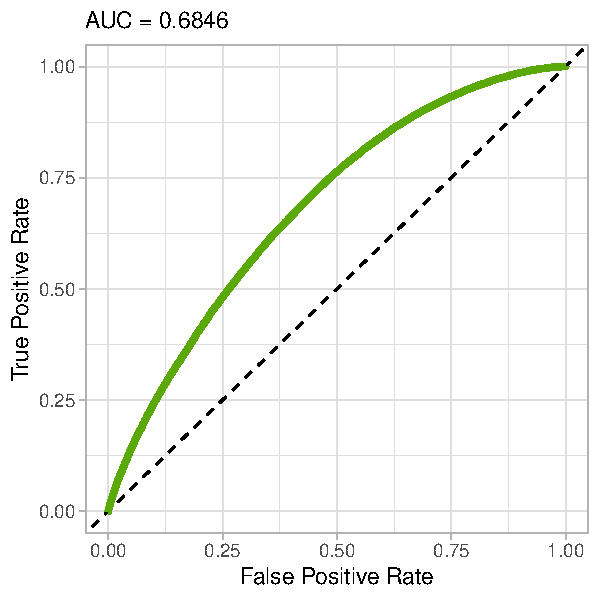
\includegraphics{report_files/figure-latex/unnamed-chunk-7-1} 

}

\caption{Receiver operating characteristic curve for CatBoost classification performance on the validation set.}\label{fig:unnamed-chunk-7}
\end{figure}

\hypertarget{feature-importance}{%
\subsection{Feature Importance}\label{feature-importance}}

After fitting the classification models, we wanted to look at how much
the models rely on the features to make predictions. Since CatBoost gave
us better classification results, we decided to look at the variable
importance obtained from this model (see Figure 6).

\begin{figure}[H]

{\centering 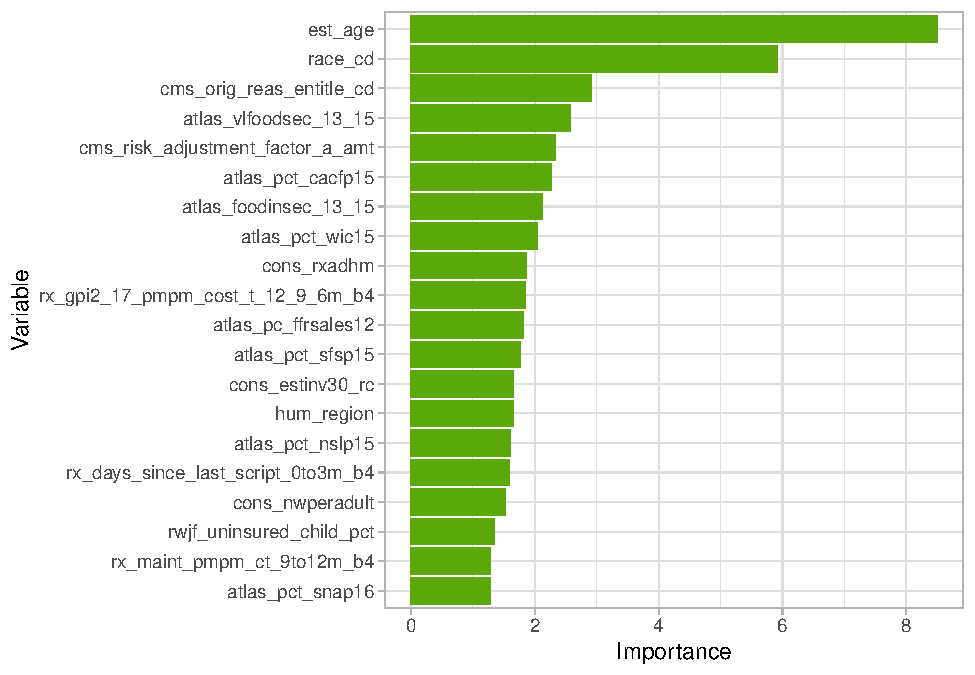
\includegraphics{report_files/figure-latex/unnamed-chunk-8-1} 

}

\caption{Top 20 important features from CatBoost model. The importance of each variable was calculated based on how much on average the prediction changes if the feature value changes.}\label{fig:unnamed-chunk-8}
\end{figure}

Table 1 gives full information about the top 20 important features from
our CatBoost model. It is clear that age is the variable that
contributes the most to the predictions of vaccination hesitancy. As we
have shown earlier in Section \ref{data}, younger member tend to have
lower vaccination rate than elderly people. In addition, race is also a
significant factor in identifying whether a member is vaccinated. We
discovered earlier that Hispanic, North American Native, and Black are
the race groups that have low vaccination rate.

\singlespacing

\small

\begin{table}[H]

\caption{\label{tab:unnamed-chunk-9}Complete descriptions of the top 20 important features obtained from CatBoost fit. These information were extracted from the data dictionary provided by the competition.}
\centering
\begin{tabular}[t]{>{\raggedright\arraybackslash}p{2in}>{\raggedright\arraybackslash}p{3.6in}}
\toprule
Feature & Description\\
\midrule
est\_age & Member age (calculated using est\_bday, relative to score/index date)\\
race\_cd & Code indicating a member's race (0 = Unknown, 1 = White, 2 = Black, 3 = Other, 4 = Asian, 5 = Hispanic, 6 = N. American Native)\\
cms\_orig\_reas \_entitle\_cd & Code indicating the original reason for entry into Medicare\\
atlas\_vlfoodsec\_13\_15 & Household very low food security (\%, three-year average), 2013-15\\
cms\_risk\_adjustment \_factor\_a\_amt & Risk Adjustment Factor A Amount\\
\addlinespace
atlas\_pct\_cacfp15 & Child \& Adult Care (\% pop)\\
atlas\_foodinsec\_13\_15 & Household food insecurity (\%, three-year average), 2013-15\\
atlas\_pct\_wic15 & WIC participants (\% pop)\\
cons\_rxadhm & RX Adherence - Maintenance\\
rx\_gpi2\_17\_pmpm\_cost \_t\_12\_9\_6m\_b4 & Trend of cost per month of prescriptions related to vaccine drugs in the past sixth to ninth month versus ninth to twelfth month prior to the score date (Based on GPI2 grouping)\\
\addlinespace
atlas\_pc\_ffrsales12 & Expenditures per capita, fast food\\
atlas\_pct\_sfsp15 & Summer Food Service Program participants (\% pop)\\
cons\_estinv30\_rc & Estimated Household Investable Assets Recoded\\
hum\_region & Member geographic information - Humana Region\\
atlas\_pct\_nslp15 & National School Lunch Program participants (\% pop)\\
\addlinespace
rx\_days\_since\_last \_script\_0to3m\_b4 & Days since last prescription in the past three
months prior to score date\\
cons\_nwperadult & Net Worth Per Adult\\
rwjf\_uninsured\_child\_pct & Clinical Care - Percentage of children under age 19
without health insurance\\
rx\_maint\_pmpm\_ct \_9to12m\_b4 & Count per month of prescriptions related to
maintenance drugs in the past ninth to twelfth
month prior to the score date\\
atlas\_pct\_snap16 & SNAP participants (\% pop)\\
\bottomrule
\end{tabular}
\end{table}

\normalsize

\doublespacing

\newpage

\hypertarget{recommendations}{%
\section{Recommendations}\label{recommendations}}

According to a recent Gallup poll of 3,572 Americans (Jones, 2021), 78\%
(of the unvaccinated surveyed) indicated that they are unlikely to or
definitely will not change their minds in receiving the COVID-19
vaccine. This provides an immense challenge to healthcare providers as
far as recommendations go, raising the question of how they can convince
non-vaccinated individuals to get the vaccine when they are already
adamant about their stance. Building a model using modern classification
techniques to predict vaccination status is only getting Humana halfway
there.

A crucial finding from Gallup's poll was that, of the unvaccinated
surveyed, 23\% cited the main reason for not getting vaccinated was they
were concerned about the safety of the vaccine. While 78\% are unlikely
to change their minds, perhaps an approach that administers positive and
accurate information and improves knowledge dissemination will allow us
to improve vaccination rate. Before considering the results of our
analysis, we would recommend Humana to mail out pamphlets related to
vaccine safety to those in their service regions to ease the main
concerns of those refusing vaccination.

Moreover, we could target these mailings to the demographic that is
currently likely to be unvaccinated. Younger people should be considered
a high priority for this initiative (see Figure 1). One possible reason
that younger people were found to be less likely to receive the vaccine
is that they do not face considerable risk to their survival and overall
well-being compared to infantile and elderly populations. Under this
hypothesis, we would also recommend that Humana identify unvaccinated
young adults and provide them with a realistic overview of the effects
of COVID-19 beyond individual harm. Instead, we should highlight the
real issues of economic pitfalls, intensive care units at capacity, and
a lack of outbreak detection in hospices that treat the elderly (Kates
et al., 2021), all of which could be avoided through vaccination.

Additionally, an essential target found in our model includes racial and
ethnic minority groups (Black, Hispanic, and Native Americans), since
these groups appeared to have relatively lower vaccination rates
compared to White and Non-Hispanic groups (see Figure 2). According to
The Centers for Disease Control and Prevention (CDC), this is due to
challenges including socioeconomic status, gaps in healthcare access,
transportation issues, lack of trust because of past medical racism and
experimentation, and other factors (CDC, 2021). In order to tackle these
challenges, that is, emphasize vaccine equity for racial and ethnic
minority groups, we suggest that Humana build rapport among their
members in these groups before even initiating to educate them. Through
this, we may have higher chances of them listening and gaining their
trust and confidence in the vaccine.

At the same time, we must empathize with those that choose not to have
themselves or their children vaccinated. Therefore, Humana should make
these messages without using phrases such as ``should get the vaccine.''
Instead, we should use diction that depicts Humana's understanding of
the concerns among unvaccinated individuals. According to a World
Economic Forum report on building trust in vaccines (World Economic
Forum, 2021), messages that make vaccines seem as if they are a moral
obligation will often evoke negative emotions. Successful messages will
not rely on morality-based arguments involving celebrities and
politicians, but rather arguments based on gratitude from healthcare
professionals or ``people like me.'' To maximize the effectiveness of
our pamphlets, Humana should incorporate these insights while making
messages regarding the protection of the elderly, the economy, the
healthcare system, and of course, those receiving the vaccine.

Another high priority target group includes members who obtain
prescriptions related to maintenance drugs in our model to predict
COVID-19 vaccination status, as these individuals contribute to a
considerable amount of our unvaccinated group. Thus, we recommend that
Humana establish a joint intervention with pharmacies, including
pamphlets supporting COVID-19 vaccination in members' prescription drug
packages. In doing so, we hope to target a large subpopulation that has
relatively low vaccination rates.

In an even greater effort to encourage the elderly to receive the
COVID-19 vaccine, we suggest that Humana targets areas such as community
centers or nursery homes in unvaccinated ``hotspot'' areas. Informative
presentations about the benefits of the vaccine, with testimonials about
COVID vaccination from their peers, could change the minds of those
refusing the vaccine, given that peer-to-peer interventions have been
shown to be effective based on a recent research from Rosenzweig et al.
(2021). In order to further strengthen this approach, Humana could offer
small incentives to those in attendance of the event, as well as reward
those who recruit others to participate. In addition to these efforts,
we recommend pre and post-surveys about COVID-19 vaccination, as a
measure of these presentations.

Along with providing this information, Humana should also send out
surveys to hone in on other reasons why people are choosing to be
unvaccinated - especially young men and those in the Black, Hispanic,
and Native American communities. These surveys could also assist in
reaching more unvaccinated Americans than we anticipate. Similar to how
the spouses of smokers are more likely to be smokers themselves
(Margolis \& Wright, 2016), we imagine that family households with one
unvaccinated family member will likely have other unvaccinated family
members in their home. Lastly, it is critical to build trust between
communities and healthcare/insurance providers. In this survey process,
it would be wise to observe whether a lack of communication is a factor
in whether or not a person is vaccinated. After determining other
various reasons for vaccine hesitancy, we can continue to update our
information to address these concerns and further educate the public on
the importance of vaccination.

\newpage

\hypertarget{conclusion}{%
\section{Conclusion}\label{conclusion}}

Humana's mission is to help people achieve lifelong well-being. COVID-19
has introduced the challenge in increasing both vaccination rates and
vaccine confidence at the forefront of minds around the world. Humana is
eager to achieve an increase in vaccination rates and vaccine confidence
among their members (especially the younger people) as well as the
larger population. Thus, for this year's case study, we developed
machine learning models that identify which members are more likely to
be hesitant to the COVID-19 vaccine.

With the provided dataset consisting of 974,842 rows and 368 columns, we
fitted gradient boosted tree models to predict vaccine hesitancy for
Humana members. Specifically, we considered two algorithms, XGBoost and
CatBoost, with CatBoost ended up being the classifier that provided the
best prediction performance. Moreover, we determined from our CatBoost
model that age and race were the two variables that have the greatest
contributions on predicting whether or not a member is vaccinated.

Based on the important features obtained from our model, we provide the
following recommendations to build confidence in the COVID-19 vaccine
and increase vaccination rates:

\begin{enumerate}
\def\labelenumi{\arabic{enumi}.}
\item
  Mail out pamphlets that summarize accurate and positive information
  related to the safety and the benefits of the vaccine.
\item
  Focus on unvaccinated young adults by providing them a realistic
  overview of the effects of COVID-19 beyond individual harm.
\item
  Build rapport among their members in the racial and ethnic minority
  groups before even initiating to educate them.
\item
  Establish a joint intervention with pharmacies by including pamphlets
  supporting COVID-19 vaccination in members' prescription drug
  packages.
\item
  Target community centers or nursery homes in unvaccinated ``hotspot''
  areas and provide an effective and informative presentation regarding
  the benefits of the vaccine.
\item
  Administer pre and post-surveys about COVID-19 vaccination, as a
  measure of effectiveness of these presentations.
\item
  Conduct surveys to obtain more information and understanding on
  COVID-19 hesitancy.
\end{enumerate}

It is imperative for healthcare and insurance providers to build a
strong relationship with the communities before even starting to inform
and educate them. With these fundamental relationships established, only
then will the public be able to invest its willingness and trust in our
healthcare agencies. And along with their trust comes the ability for
the community to achieve Humana's mission of lifelong well-being.

\newpage

\hypertarget{references}{%
\section*{References}\label{references}}
\addcontentsline{toc}{section}{References}

\hypertarget{refs}{}
\begin{CSLReferences}{1}{0}
\leavevmode\vadjust pre{\hypertarget{ref-cdc}{}}%
CDC. (2021). \emph{COVID-19 vaccine equity for racial and ethnic
minority groups}.
\url{https://www.cdc.gov/coronavirus/2019-ncov/community/health-equity/vaccine-equity.html}

\leavevmode\vadjust pre{\hypertarget{ref-xgpaper}{}}%
Chen, T., \& Guestrin, C. (2016). XGBoost: A scalable tree boosting
system. \emph{Proceedings of the 22nd ACM SIGKDD International
Conference on Knowledge Discovery and Data Mining}, 785--794.
\url{https://doi.org/10.1145/2939672.2939785}

\leavevmode\vadjust pre{\hypertarget{ref-xgpackage}{}}%
Chen, T., He, T., Benesty, M., Khotilovich, V., Tang, Y., Cho, H., Chen,
K., Mitchell, R., Cano, I., Zhou, T., Li, M., Xie, J., Lin, M., Geng,
Y., \& Li, Y. (2021). \emph{Xgboost: Extreme gradient boosting}.
\url{https://CRAN.R-project.org/package=xgboost}

\leavevmode\vadjust pre{\hypertarget{ref-gallup}{}}%
Jones, J. M. (2021). \emph{COVID-19 vaccine-reluctant in u.s. Likely to
stay that way}.
\url{https://news.gallup.com/poll/350720/covid-vaccine-reluctant-likely-stay.aspx}

\leavevmode\vadjust pre{\hypertarget{ref-impact}{}}%
Kates, J., Gerolamo, A., \& Pogorzelska-Maziarz, M. (2021). {{T}he
impact of {C}{O}{V}{I}{D}-19 on the hospice and palliative care
workforce}. \emph{Public Health Nurs}, \emph{38}(3), 459--463.

\leavevmode\vadjust pre{\hypertarget{ref-tidymodels}{}}%
Kuhn, M., \& Wickham, H. (2020). \emph{Tidymodels: A collection of
packages for modeling and machine learning using tidyverse principles.}
\url{https://www.tidymodels.org}

\leavevmode\vadjust pre{\hypertarget{ref-smokers}{}}%
Margolis, R., \& Wright, L. (2016). {{B}etter {O}ff {A}lone {T}han
{W}ith a {S}moker: {T}he {I}nfluence of {P}artner's {S}moking {B}ehavior
in {L}ater {L}ife}. \emph{J Gerontol B Psychol Sci Soc Sci},
\emph{71}(4), 687--697.

\leavevmode\vadjust pre{\hypertarget{ref-cbpaper}{}}%
Prokhorenkova, L., Gusev, G., Vorobev, A., Dorogush, A. V., \& Gulin, A.
(2018). CatBoost: Unbiased boosting with categorical features.
\emph{Proceedings of the 32nd International Conference on Neural
Information Processing Systems}, 6639--6649.
\url{https://dl.acm.org/doi/abs/10.5555/3327757.3327770}

\leavevmode\vadjust pre{\hypertarget{ref-rcite}{}}%
R Core Team. (2021). \emph{R: A language and environment for statistical
computing}. R Foundation for Statistical Computing.
\url{https://www.R-project.org/}

\leavevmode\vadjust pre{\hypertarget{ref-medicare}{}}%
ResDAC. (2021). \emph{Original reason for entitlement code}.
\url{https://resdac.org/cms-data/variables/original-reason-entitlement-code}

\leavevmode\vadjust pre{\hypertarget{ref-peer}{}}%
Rosenzweig, L. R., Platas, M. R., \& Bicalho, C. (2021).
\emph{Peer-to-peer communication in east and west africa may help
promote COVID-19 policy compliance}.
\url{https://blogs.lse.ac.uk/africaatlse/2021/04/21/peer-communication-east-west-africa-help-promote-covid19-health-policy-compliance/}

\leavevmode\vadjust pre{\hypertarget{ref-trust}{}}%
World Economic Forum. (2021). \emph{How to build trust in vaccines:
Understanding the drivers of vaccine confidence}.
\url{https://www.weforum.org/reports/how-to-build-trust-in-vaccines-understanding-the-drivers-of-vaccine-confidence}

\end{CSLReferences}

\end{document}
